%% ServiceScope: Pre-Deployment Inter-Service Dependency Mapping
%% via AST Analysis and Local LLM Inference
%% FTC 2026 Late-Breaking Round — Double-Blind Submission
%% Springer LNCS/LNNS Format

\documentclass[runningheads]{llncs}

\usepackage[T1]{fontenc}
\usepackage{graphicx}
\usepackage{booktabs}
\usepackage{multirow}
\usepackage{amsmath}
\usepackage{amssymb}
\usepackage{xcolor}
\usepackage{listings}
\usepackage{microtype}
\usepackage{array}
\usepackage{tabularx}
\usepackage{tikz}
\usetikzlibrary{shapes.geometric,arrows.meta,positioning,fit,backgrounds}
\usepackage{hyperref}  % must be last

\lstset{
  basicstyle=\ttfamily\small,
  breaklines=true,
  frame=single,
  numbers=left,
  numberstyle=\tiny,
}

\begin{document}

\title{ServiceScope: Pre-Deployment Inter-Service Dependency Mapping
via Multi-Language AST Analysis and Local LLM Inference}

%% Double-blind: author block omitted for review
\author{Anonymous}
\institute{Anonymous Institution}

\maketitle

% ─────────────────────────────────────────────────────────────────────────────
\begin{abstract}
Understanding inter-service dependencies before deployment is a critical yet
unsolved challenge in microservice development. Existing approaches rely on
runtime instrumentation, manual catalogues, or commit-history coupling---none
of which operate on source code alone prior to deployment. A key barrier is
\emph{dynamic URL resolution}: the majority of inter-service HTTP and gRPC
calls reference variable names rather than hardcoded strings, making pure
static analysis completely blind to them.

We present \textsc{ServiceScope}, the first static analysis pipeline that
combines AST-based HTTP and gRPC call extraction with local LLM inference to
resolve dynamic variable names into service identities---without runtime
agents or external API calls. The system supports Python and Go codebases and
produces a confidence-weighted inter-service dependency graph from which
pre-deployment blast radius predictions are computed via Dijkstra-based
transitive closure.

We evaluate \textsc{ServiceScope} across five benchmark repositories (three
Python, two Go) spanning 6 LLMs, 4 prompting configurations, and two
protocols. AST extraction achieves F1\,=\,1.000 on all repositories after
false-positive guards. Inference F1 ranges from 0.000 (generic variable
names, irreducible ceiling) to 1.000 (descriptive variable names), with
service-aware prompting reaching F1\,=\,0.455 on a complex polyglot
repository where the static baseline scores 0.000. Blast radius precision
reaches 0.374 versus 0.000 for static analysis. We further validate the
system on \emph{argoproj/argo-cd} (18k GitHub stars), correctly recovering
all three core architecture edges published in the official documentation.
\end{abstract}

\keywords{microservices \and static analysis \and dependency mapping \and
large language models \and blast radius \and pre-deployment}

% ─────────────────────────────────────────────────────────────────────────────
\section{Introduction}
\label{sec:intro}

Modern software systems decompose business logic across tens to hundreds of
independently deployable microservices~\cite{dragoni2017,fowler2014,newman2021}. A fundamental operational challenge
arises when a developer modifies one service: \emph{which other services
will be affected?} This question---the \emph{blast radius} of a
change---determines testing scope, rollout risk, and incident response
priority. Yet answering it before deployment remains largely manual or
entirely absent in most engineering workflows.

Existing dependency discovery tools partition into three classes, each with
a critical gap. Runtime tracers such as Datadog~\cite{datadog}, Jaeger, and
Instana construct accurate service maps but require deployed infrastructure
and post-deployment observation---unavailable during code review or in
pre-production environments. Manual catalogues such as Backstage~\cite{backstage}
are accurate when maintained but drift from the codebase silently as
services evolve. Change-coupling tools such as CodeScene infer relationships
from commit history rather than code structure, requiring a substantial
commit corpus and providing coupling statistics rather than architectural
truth.

The closest academic prior work, Microvision~\cite{cerny2022}, reconstructs
inter-service REST call graphs via AST analysis but is restricted to static
URL strings and Java/Spring Boot codebases. It cannot handle dynamic URL
patterns and provides no blast radius computation.

A key obstacle all static approaches share is \emph{dynamic URL resolution}.
In practice, inter-service calls rarely use hardcoded URLs. Instead, they
reference environment variables, configuration constants, or computed
strings---for example, \texttt{requests.get(PAYMENT\_SERVICE\_URL)} or
\texttt{grpc.Dial(os.Getenv("CART\_SERVICE\_ADDR"))}. A static analyser
that sees only these variable names cannot identify the target service
without additional inference.

\textsc{ServiceScope} addresses this gap. Our contributions are:

\begin{enumerate}
  \item A multi-language AST extractor covering eight Python and four Go
    HTTP/gRPC call patterns, with false-positive guards verified on real
    repositories (\S\ref{sec:extraction}).
  \item A four-phase LLM inference pipeline that resolves dynamic variable
    names to service identities using local Ollama models---no external API
    calls, no deployed infrastructure (\S\ref{sec:llm}).
  \item A service-aware prompting technique that constrains LLM output to
    the repository's known service inventory, reducing hallucinated names
    and doubling inference F1 on complex repositories (\S\ref{sec:llm}).
  \item A confidence-weighted blast radius computation via log-space
    Dijkstra traversal with bidirectional transitive closure (\S\ref{sec:blast}).
  \item An empirical evaluation across five repositories, six LLMs, and four
    prompting configurations, with an independent verification on a
    production-grade open-source system (\S\ref{sec:eval}).
\end{enumerate}

\subsection{Scope and Assumptions}
\label{sec:scope}

For this study, a \emph{service} is defined as a distinct directory
containing an independent executable entry point (e.g., \texttt{main.py},
\texttt{main.go}, or a framework-specific application factory) alongside
its own dependency manifest (e.g., \texttt{go.mod},
\texttt{requirements.txt}, \texttt{package.json}). This definition
structurally distinguishes deployable, self-contained microservices from
shared internal libraries, utility modules, or orphaned scripts.

\textsc{ServiceScope} assumes a \emph{monorepo} layout in which all
services reside under a common root directory. Polyrepo configurations---in
which each service occupies an independent repository---are outside the
scope of this work; extending the system to polyrepo layouts requires only
a repository aggregation step upstream of the extraction pipeline. The term
\emph{pre-deployment} refers to any point in the development lifecycle
prior to execution in a staging or production environment, encompassing
local development, code review, and CI/CD pipeline stages.

% ─────────────────────────────────────────────────────────────────────────────
\section{Related Work}
\label{sec:related}

\subsection{Runtime and Dynamic Instrumentation Approaches}

Service mesh and APM tools---Datadog~\cite{datadog}, Jaeger, Instana,
Zipkin, and service meshes such as Istio~\cite{istio}---instrument deployed
services to trace actual call flows. They
produce highly accurate dependency maps but require running infrastructure.
Their fundamental limitation is temporal: they cannot answer dependency
questions before a service is deployed or when a production environment is
unavailable. \textsc{ServiceScope} operates entirely on source code,
complementing these tools rather than replacing them.

\subsection{Static and Heuristic Approaches}

Microvision~\cite{cerny2022} is the closest prior work. It reconstructs
inter-service REST call graphs from Java source code using AST analysis of
Spring Boot annotations. Its scope is limited to static URL strings;
dynamic URL patterns are outside its design. It provides no LLM inference
layer and no blast radius computation. Backstage~\cite{backstage} is a
service catalogue requiring human-authored YAML descriptors; it is accurate
only when manually kept in sync with the codebase. CodeScene~\cite{codescene} infers service coupling from co-change patterns
in git history, requiring an extensive commit corpus and producing
statistical correlation rather than structural dependency. These approaches collectively demonstrate that
static analysis of source code is under-explored for pre-deployment
dependency mapping.

\subsection{LLM-Assisted Software Engineering}

Large language models have been applied broadly to software engineering
tasks. CodeBERT~\cite{codebert} established that pre-trained models can
jointly represent programming and natural language, enabling tasks such as
code search and clone detection. Subsequent surveys~\cite{zhu2023survey,fan2023llmse}
document LLM applications across bug detection, code generation, test
synthesis, and code summarisation. Critically, none of these works targets
inter-service dependency mapping; they operate at the function or file
level rather than the architectural level. \textsc{ServiceScope} is, to our
knowledge, the first application of LLM inference specifically to resolve
dynamic service-call targets in a multi-language static analysis pipeline.

% ─────────────────────────────────────────────────────────────────────────────
\section{System Architecture}
\label{sec:arch}

\begin{figure}[t]
\centering
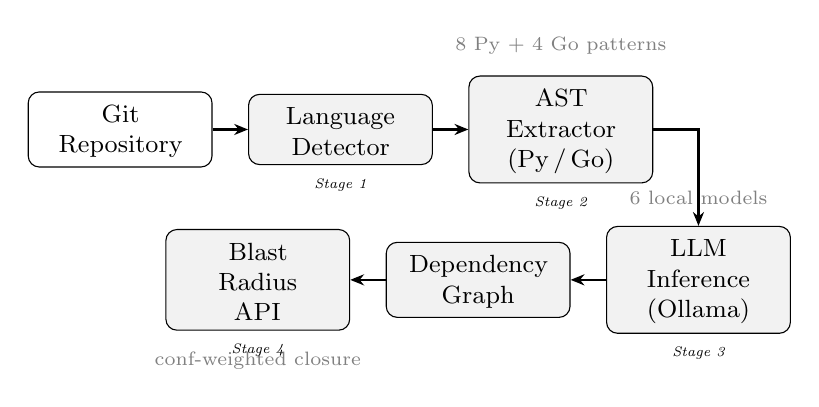
\begin{tikzpicture}[
  box/.style={
    rectangle, rounded corners=4pt,
    draw=black, fill=gray!10,
    text width=2.1cm, minimum height=0.85cm,
    align=center, font=\small\strut
  },
  wbox/.style={
    rectangle, rounded corners=4pt,
    draw=black, fill=white,
    text width=2.1cm, minimum height=0.85cm,
    align=center, font=\small\strut
  },
  arr/.style={-{Stealth[length=5pt,width=4pt]}, thick},
  node distance=0.55cm and 0.45cm,
]

%% ── Row 1 (left → right) ──────────────────────────────────────────
\node[wbox]                      (repo)   {Git\\Repository};
\node[box, right=of repo]        (lang)   {Language\\Detector};
\node[box, right=of lang]        (ast)    {AST\\Extractor\\(Py\,/\,Go)};

%% ── Connector node (invisible) for the bend ──────────────────────
\node[right=0.45cm of ast]       (bend)   {};

%% ── Row 2 (right → left) ──────────────────────────────────────────
\node[box, below=1.1cm of bend]  (llm)    {LLM\\Inference\\(Ollama)};
\node[box, left=of llm]          (graph)  {Dependency\\Graph};
\node[box, left=of graph]        (blast)  {Blast\\Radius\\API};

%% ── Annotations ──────────────────────────────────────────────────
\node[above=0.15cm of ast,  font=\scriptsize, text=gray]
      {8 Py + 4 Go patterns};
\node[above=0.15cm of llm,  font=\scriptsize, text=gray]
      {6 local models};
\node[below=0.15cm of blast, font=\scriptsize, text=gray]
      {conf-weighted closure};

%% ── Arrows row 1 ─────────────────────────────────────────────────
\draw[arr] (repo)  -- (lang);
\draw[arr] (lang)  -- (ast);
\draw[arr] (ast)   -- (bend.center) -- ++(0,-0.55) -- (llm.north);

%% ── Arrows row 2 ─────────────────────────────────────────────────
\draw[arr] (llm)   -- (graph);
\draw[arr] (graph) -- (blast);

%% ── Stage labels ─────────────────────────────────────────────────
\node[font=\tiny\itshape, below=0.05cm of lang]  {Stage 1};
\node[font=\tiny\itshape, below=0.05cm of ast]   {Stage 2};
\node[font=\tiny\itshape, below=0.05cm of llm]   {Stage 3};
\node[font=\tiny\itshape, below=0.05cm of blast] {Stage 4};

\end{tikzpicture}
\caption{The \textsc{ServiceScope} four-stage pipeline. A cloned
  repository passes through language detection, AST extraction, local LLM
  inference, and graph-based blast radius computation.}
\label{fig:pipeline}
\end{figure}

\textsc{ServiceScope} processes a repository in four sequential stages,
shown in Fig.~\ref{fig:pipeline}.

\textbf{Stage 1 --- Language Detection.} The repository root is scanned to
identify Python (\texttt{.py}) and Go (\texttt{.go}) source files. Service
boundaries are determined according to the definition in \S\ref{sec:scope}.

\textbf{Stage 2 --- AST Extraction.} Language-specific extractors traverse
the abstract syntax tree of each source file, identifying HTTP and gRPC
call sites. Static URL strings are recorded directly; dynamic references
are encoded as \texttt{<dynamic:VAR\_NAME>} tokens carrying the variable
name for downstream inference. Full pattern details are given in
\S\ref{sec:extraction}.

\textbf{Stage 3 --- LLM Inference.} Each extracted call is submitted to a
local Ollama instance. The LLM maps the variable name or URL pattern to a
target service name and returns a confidence score. Inference operates
entirely locally---no external API calls are required, making the tool
suitable for air-gapped or privacy-sensitive environments. Prompt design
and the four-phase configuration are described in \S\ref{sec:llm}.

\textbf{Stage 4 --- Graph Construction and Blast Radius.} Inferred
dependencies are assembled into a directed weighted graph. Blast radius for
a given service is computed as the confidence-weighted transitive closure
via bidirectional Dijkstra traversal (\S\ref{sec:blast}).

% ─────────────────────────────────────────────────────────────────────────────
\section{Multi-Language AST Extraction}
\label{sec:extraction}

\subsection{Python Extractor}

The Python extractor implements eight call patterns using the \texttt{ast}
module. Patterns 1--5 target the \texttt{requests}, \texttt{httpx},
\texttt{aiohttp}, and \texttt{urllib} libraries. Pattern~6 handles f-string
URL construction by extracting the static prefix. Patterns~7 and~8 capture
variable-based and concatenated URLs, encoding them as dynamic tokens.

A critical false-positive guard---\texttt{require\_absolute=True}---is
applied to generic \texttt{client.get/post()} calls (Pattern~3). Without
this guard, dictionary lookups (\texttt{metrics.get("cpu")}) and
queue operations (\texttt{workers.get()}) are misclassified as HTTP
calls. On \emph{robusta-dev/robusta}, this guard reduced false positives
from 81.5\% to 0\% of extracted calls.

\subsection{Go Extractor}

The Go extractor is implemented as a Go binary using the \texttt{go/ast}
and \texttt{go/parser} standard library packages, invoked via a Python
subprocess wrapper. It resolves four call patterns: \texttt{net/http}
method calls, gRPC \texttt{Dial}/\texttt{NewClient} invocations,
\texttt{os.Getenv} address lookups, and---critically---custom client
constructor calls of the form \texttt{apiclient.New*Clientset(address)}.

The fourth pattern addresses a pervasive Go architectural convention in
which gRPC connections are wrapped in factory functions. Without it, the
extractor registers calls under the helper package rather than the true
initiator. Adding constructor-call extraction enabled \textsc{ServiceScope}
to correctly map all three core architecture edges in
\emph{argoproj/argo-cd} (\S\ref{sec:eval}).

\subsection{Inter-Procedural Ceiling}

Both extractors operate \emph{intra-procedurally}: they analyse each
function body independently. A well-documented class of Go microservice
patterns wraps connection setup in helper functions, for example:

\begin{lstlisting}[language=Go, caption={}]
mustConnGRPC(ctx, &conn, os.Getenv("CART_SERVICE_ADDR"))
\end{lstlisting}

The extractor sees \texttt{CART\_SERVICE\_ADDR} inside the helper body but
cannot link it back to the calling service without cross-function data-flow
analysis. This constitutes an irreducible ceiling for intra-procedural
static analysis, discussed as a threat to external validity in
\S\ref{sec:discussion}.

\subsection{Polyglot Service Discovery}

Service-aware prompting (\S\ref{sec:llm}) requires a list of known service
names prior to inference. The discovery step scans the repository root for
subdirectories satisfying the service definition (\S\ref{sec:scope}).
Crucially, eligibility is determined by the \emph{presence of any source
files}---not only \texttt{.py} or \texttt{.go}---so that Java, C\#, and
Node.js service directories in polyglot repositories are included. A fixed
ignore list excludes non-service directories such as \texttt{tests},
\texttt{docs}, \texttt{vendor}, and \texttt{node\_modules}.

% ─────────────────────────────────────────────────────────────────────────────
\section{LLM Inference Pipeline}
\label{sec:llm}

\subsection{Model Selection}

We evaluate six locally-hosted models spanning four orders of magnitude in
parameter count, from \texttt{qwen2.5:1.5b} (986\,MB) to
\texttt{gemma4:latest} (9.6\,GB). The set includes general-purpose models
(\texttt{gemma3:4b}, \texttt{llama3.1:8b}, \texttt{gemma4:latest}), a
code-specialised model (\texttt{qwen2.5-coder:7b}), a compact general
model (\texttt{qwen2.5:1.5b}), and a reasoning model (\texttt{qwen3:4b}).
Full model specifications are provided in Appendix~\ref{app:models}.

\subsection{Four-Phase Prompt Design}
\label{sec:phases}

Inference accuracy was improved through four successive prompt
configurations:

\textbf{Phase~1 --- Static Baseline.} Regex-based hostname extraction from
hardcoded URL strings. No LLM involved. Returns \texttt{null} for any
dynamic call.

\textbf{Phase~2 --- Zero-Shot Inference.} The LLM receives caller service
name, HTTP method, and URL or variable name. It returns a JSON object with
\texttt{service} and \texttt{confidence} fields. No examples are provided.

\textbf{Phase~3 --- Suffix-Normalised Evaluation.} Predicted service names
are normalised by stripping a locked set of architectural suffixes
(\texttt{\_service}, \texttt{\_client}, \texttt{\_api}, \texttt{\_handler},
\texttt{\_server}, \texttt{\_svc}) before string matching. This phase does
not change the prompt; it corrects for systematic suffix mismatch between
model output and ground truth labels.

\textbf{Phase~4 --- Service-Aware Prompting.} Before inference, the service
discovery step produces a list of known service names in the repository.
This list is injected into the prompt, converting the task from
unconstrained generation to constrained selection. An external service
escape hatch instructs the model to return the external API name if no
known service matches. Prompt templates are given in Appendix~\ref{app:prompts}.

\subsection{Engineering Notes}

\textbf{Reasoning model handling.} \texttt{qwen3:4b} is a distilled
reasoning model that outputs chain-of-thought to a \texttt{thinking} field,
leaving the \texttt{response} field empty. The inference client falls back
to the \texttt{thinking} field when \texttt{response} is absent, enabling
transparent support for both standard and reasoning model architectures.

\textbf{Negative few-shot bias.} Including few-shot examples that
demonstrate the \texttt{unknown} fallback for generic variable names
(\texttt{<dynamic:url> $\to$ unknown}) creates a strong conservative prior.
All models score F1\,=\,0.000 in few-shot mode on both Go repositories,
whereas zero-shot achieves up to 0.400. We therefore report few-shot
results only for Python repositories where examples improve performance.

\textbf{Service-aware prompting on monolith layouts.} On repositories with
a monolith-style directory structure (e.g., \emph{robusta-dev/robusta}),
directory scanning yields internal package names rather than service names.
Injecting these as the known service list confuses the LLM and degrades
performance (F1 drops from 0.267 to 0.056). Service-aware prompting should
therefore be applied only when directory structure reflects genuine service
boundaries.

\textbf{Computational overhead.} Per-call inference latency ranges from
383\,ms (\texttt{qwen2.5:1.5b}) to 4.6\,s (\texttt{gemma4:latest}).
On the largest benchmark repository (35 calls), the full pipeline completes
in under 60\,s on consumer hardware (Apple Silicon, OLLAMA\_NUM\_PARALLEL=4),
making it practical for integration into pre-merge CI workflows.

% ─────────────────────────────────────────────────────────────────────────────
\section{Blast Radius Computation}
\label{sec:blast}

\subsection{Graph Model}

Inferred dependencies are represented as a directed weighted graph
$G = (V, E, w)$ where nodes $V$ are normalised service names, directed
edges $E$ represent inferred call relationships, and weight function
$w: E \to [0,1]$ carries the LLM confidence score. When multiple calls
exist between the same pair of services, the edge retains the maximum
confidence across all calls.

\subsection{Confidence Propagation}

Treating each LLM inference as an independent event, the confidence of a
path $\pi = (e_1, e_2, \ldots, e_k)$ is the product of edge confidences:

\begin{equation}
  P(\pi) = \prod_{i=1}^{k} w(e_i)
\end{equation}

To find the maximum-confidence path from source service $s$ to any
reachable service $t$, we apply Dijkstra's algorithm in log-space:
edge weight $w(e)$ is transformed to $-\log(w(e) + \varepsilon)$, where
$\varepsilon = 10^{-9}$ prevents numerical underflow for zero-confidence
edges. Standard shortest-path minimisation then maximises the product of
original confidences.

\subsection{Bidirectional Traversal}

Blast radius encompasses two directions of impact. \emph{Outbound impact}
(services that $X$ calls) captures dependencies that may receive altered
inputs if $X$ changes. \emph{Inbound impact} (services that call $X$)
captures callers whose behaviour may break if $X$'s API changes. Two
separate Dijkstra traversals are performed---one on $G$, one on the
reversed graph $G^R$---and results are merged, deduplicating any service
appearing in both directions and annotating it as bidirectionally affected.

\subsection{API}

The blast radius endpoint accepts a service name and a minimum confidence
threshold:

\begin{verbatim}
GET /api/v1/repositories/{id}/blast-radius
    ?service=X&min_confidence=0.5
\end{verbatim}

The response lists each affected service with its direction, hop count,
path, and path confidence. Services with path confidence below the threshold
are excluded.

\begin{figure}[t]
  \centering
  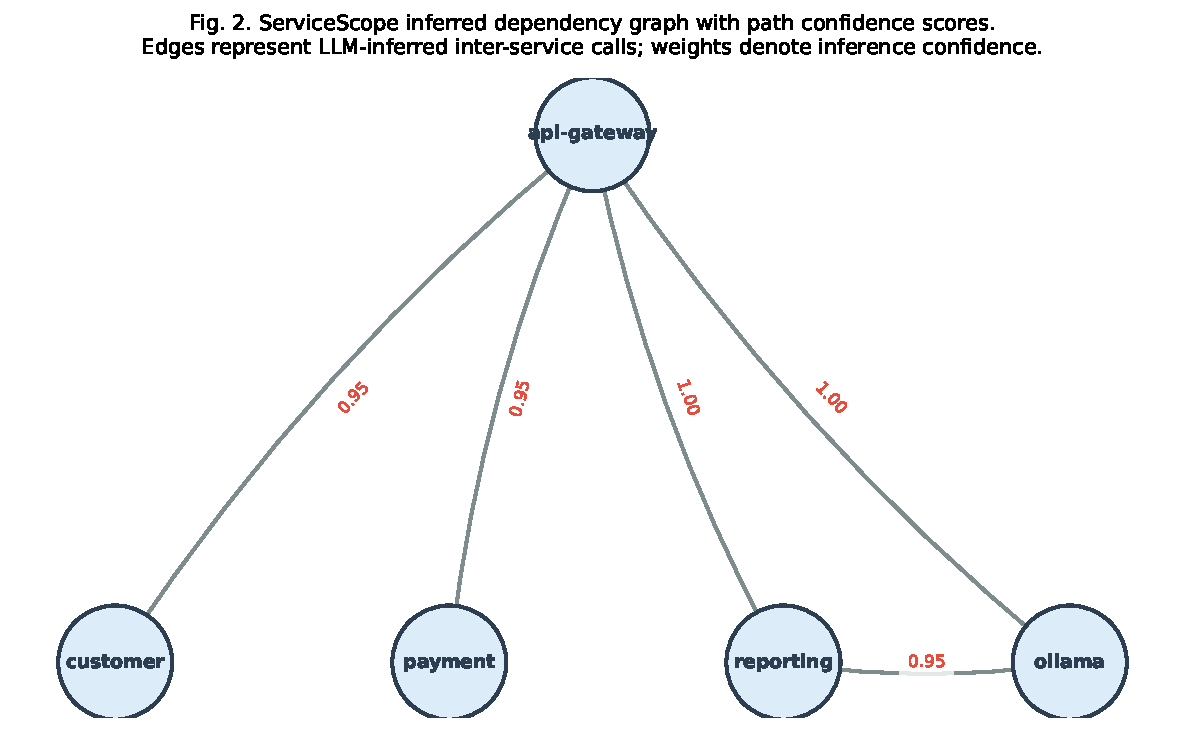
\includegraphics[width=0.85\linewidth]{figures/servicescope_v1_graph.pdf}
  \caption{\textsc{ServiceScope} inferred dependency graph for the
    case study repository. Edge labels denote LLM inference confidence;
    all edges were verified against ground truth.}
  \label{fig:graph}
\end{figure}

Fig.~\ref{fig:graph} shows the dependency graph for the case study
repository (five services, five verified edges). With \texttt{api-gateway}
as the blast radius source, all four downstream services are recovered at
path confidence $\geq 0.95$.

% ─────────────────────────────────────────────────────────────────────────────
\section{Evaluation}
\label{sec:eval}

\subsection{Dataset Construction and Ground Truth}
\label{sec:gt}

We evaluate on five repositories selected to represent diverse architectural
topologies across two languages, three protocols, and five distinct naming
convention profiles (Table~\ref{tab:repos}).

\begin{table}[t]
\caption{Benchmark repositories. GT = ground truth source.}
\label{tab:repos}
\centering
\small
\begin{tabular}{llllcc}
\toprule
\# & Repository & Lang & Protocol & Calls & GT Source \\
\midrule
1 & \emph{karpathy/nanochat} & Py & HTTP & 3 & Manual \\
2 & \emph{robusta-dev/robusta} & Py & HTTP & 35 & Manual \\
3 & Case study repository & Py & HTTP & 5 & Authors \\
4 & \emph{thangchung/go-coffeeshop} & Go & HTTP/gRPC & 3 & Manual \\
5 & \emph{microservices-demo} & Go/Py & gRPC & 7 & Arch. diagram \\
\bottomrule
\end{tabular}
\end{table}

Ground truth files were constructed independently of the extractor.
An initial evaluation revealed that an earlier version of the nanochat and
robusta ground truth files had been derived from extractor output, creating
a circular evaluation. This was corrected via independent manual inspection
using ripgrep to enumerate all HTTP call sites. The corrected ground truth
for \emph{robusta-dev/robusta} increased the true call count from 19 to 35,
revealing that the extractor had missed attribute-access patterns
(\texttt{self.url}, \texttt{action\_params.url}) and a \texttt{urllib}
ordering bug. Both issues were fixed prior to evaluation.

We defend the dataset size not by quantity but by \emph{topological
diversity}: generic-naming Python (nanochat), monolith-style Python
(robusta), descriptive-naming Python (case study), clean Go gRPC
(go-coffeeshop), and complex polyglot gRPC (microservices-demo). Each
repository exercises a distinct failure mode of the extraction and inference
pipeline.

\subsection{Metrics}

Extraction accuracy is measured as precision, recall, and F1 over the set
of (caller, method, file) triples. Inference accuracy is measured as
precision, recall, and F1 over the set of (caller, callee) dependency pairs,
after applying the locked suffix normaliser. All results are reported at the
best-performing model and configuration per repository per phase.

\subsection{Extraction Accuracy}

The AST extractor achieves F1\,=\,1.000 on all five repositories after the
false-positive guards and urllib bug fix described in \S\ref{sec:gt}. This
result is non-trivial: earlier versions of the extractor scored F1 below
0.50 on repositories with attribute-access patterns, and exhibited an 81.5\%
false-positive rate on robusta due to unguarded generic \texttt{.get()}
calls.

\subsection{Inference Accuracy: Four-Phase Progression}

Table~\ref{tab:inference} reports the best inference F1 per repository
across the four pipeline phases.

\begin{table}[t]
\caption{Best inference F1 per repository across four pipeline phases.
  SA = service-aware; ZS = zero-shot; FS = few-shot.}
\label{tab:inference}
\centering
\small
\begin{tabular}{lccccl}
\toprule
Repository & Ph.1 & Ph.2 & Ph.3 & Ph.4 & Best Config \\
\midrule
nanochat          & 0.000 & 0.000 & 0.000 & 0.000 & --- (ceiling) \\
robusta           & 0.000 & 0.167 & 0.267 & 0.188 & qwen3:4b ZS \\
Case study repo   & 0.200 & 0.800 & 1.000 & 0.800 & gemma4 ZS \\
go-coffeeshop     & 0.000 & 0.333 & 0.400 & 0.400 & qwen2.5:1.5b ZS \\
microservices-demo & 0.000 & 0.091 & 0.182 & \textbf{0.455} & llama3.1:8b SA \\
\bottomrule
\end{tabular}
\end{table}

The static baseline (Phase~1) returns F1\,=\,0.000 on four of five
repositories, confirming that dynamic variable names are the dominant call
pattern in real-world microservice code. Phase~2 introduces LLM inference
and recovers a measurable fraction of dependencies on all repositories
except nanochat. Phase~3 normalisation improves F1 uniformly by correcting
systematic suffix mismatch. Phase~4 service-aware prompting yields the
largest single gain on microservices-demo (0.182$\to$0.455), where the
constrained selection task replaces unconstrained name generation; it
regresses on robusta due to monolith directory structure as discussed in
\S\ref{sec:llm}.

\subsection{Model Ablation}
\label{sec:ablation}

Three cross-cutting findings emerge from the model ablation (full tables in
Appendix~\ref{app:ablation}):

\textbf{Reasoning models prefer zero-shot.} \texttt{qwen3:4b} scores
F1\,=\,0.167 (zero-shot) versus F1\,=\,0.071 (few-shot) on robusta, the
reverse of the pattern for all other models. Its strong instruction-following
causes few-shot examples to anchor output format in a way that suppresses
valid variable-name signal.

\textbf{Few-shot prompting backfires on Go repositories.} All models score
F1\,=\,0.000 in few-shot mode on both Go repositories. The few-shot
examples were constructed from Python naming conventions; on Go codebases
with environment-variable address patterns, these examples actively mislead
the model.

\textbf{Code-specialised models do not consistently outperform general
models.} \texttt{qwen2.5-coder:7b} achieves comparable or lower F1 than
\texttt{llama3.1:8b} on three of five repositories, suggesting that
service-name inference from variable names is not primarily a code
comprehension task.

\subsection{Blast Radius Accuracy}

Table~\ref{tab:blast} reports blast radius precision, recall, and F1
computed against ground-truth dependency graphs on two repositories.

\begin{table}[t]
\caption{Blast radius evaluation: static baseline vs.\ zero-shot
  LLM vs.\ service-aware (SA) LLM inference.}
\label{tab:blast}
\centering
\small
\begin{tabular}{llccc}
\toprule
Repository & Config & P & R & F1 \\
\midrule
\multirow{3}{*}{microservices-demo}
  & Static   & 0.000 & 0.000 & 0.000 \\
  & Zero-shot & 0.250 & 0.098 & 0.133 \\
  & SA        & 0.392 & 0.463 & \textbf{0.374} \\
\midrule
\multirow{2}{*}{Case study repo}
  & Static   & 0.190 & 0.190 & 0.190 \\
  & LLM      & 1.000 & 1.000 & \textbf{1.000} \\
\bottomrule
\end{tabular}
\end{table}

On microservices-demo, the static baseline is entirely blind (F1\,=\,0.000)
because all gRPC addresses are dynamic. Service-aware LLM inference
recovers F1\,=\,0.374---a result achievable only through dynamic variable
resolution. The blast radius F1 is lower than the inference F1 (0.374
vs.\ 0.455) because transitive closure compounds inference errors: a missed
direct edge removes all downstream services from the predicted affected set.

Path confidence calibration is reported exploratorily given sample size
constraints. In the 0.90--1.00 band, 61.5\% of predicted blast radius edges
appear in the ground truth ($n\,=\,26$). In the 0.80--0.90 band, accuracy
falls to 33.3\% ($n\,=\,6$), indicating systematic overconfidence in this
range. Users should interpret confidence scores as relative rankings rather
than absolute probabilities.

\subsection{Verification on a Production System}
\label{sec:argocd}

To assess scalability to production-grade systems, we ran
\textsc{ServiceScope} on \emph{argoproj/argo-cd}~\cite{argocd}
(\textasciitilde18k GitHub stars), a widely deployed Kubernetes GitOps
controller. Service discovery identified 26 component directories. Using
service-aware zero-shot inference (\texttt{llama3.1:8b}), the system
produced 14 directed dependency edges.

We verified the three core inter-service connections against the official
Argo CD architecture documentation~\cite{argocd-arch}:

\begin{itemize}
  \item \texttt{argocd-server} $\to$ \texttt{argocd-repo-server} (gRPC, conf=1.00) \checkmark
  \item \texttt{argocd-application-controller} $\to$ \texttt{argocd-repo-server} (gRPC, conf=1.00) \checkmark
  \item \texttt{argocd-server} $\to$ \texttt{argocd-application-controller} (gRPC, conf=1.00) \checkmark
\end{itemize}

All three published connections were recovered with zero false positives
among the core service set. This result required extending the Go extractor
with a constructor-call pattern (\texttt{apiclient.New*Clientset}), which
generalises to any Go codebase using factory functions to wrap gRPC clients.
No ground truth was available for the remaining 11 inferred edges; they are
excluded from quantitative evaluation.

% ─────────────────────────────────────────────────────────────────────────────
\section{Discussion and Threats to Validity}
\label{sec:discussion}

\subsection{Construct Validity}

\textbf{Are we measuring the right things?} F1 over (caller, callee) pairs
assumes that service name identity is the correct unit of evaluation. In
practice, service names in source code are not always canonical: a service
may be called \texttt{payment-service}, \texttt{payment\_svc}, or
\texttt{billing} across different files. The locked suffix normaliser
mitigates this but does not fully resolve it. Confidence calibration is
reported exploratorily; with five benchmark repositories and 30--40 total
blast radius edges, per-band sample sizes are insufficient for statistical
confidence intervals.

\subsection{Internal Validity}

\textbf{Confounding factors.} The negative few-shot bias demonstrates
that prompt design choices interact with model architecture in non-obvious
ways. The performance regression of service-aware prompting on monolith
repositories shows that the effectiveness of a prompting strategy is
dependent on repository structure. These interactions are documented as
experimental observations but a controlled study isolating each factor
independently is left for future work.

\subsection{External Validity}

\textbf{Naming specificity ceiling.} The most fundamental limitation of
any static analysis approach is irreducible: when a variable is named
\texttt{url}, no amount of inference recovers its target without runtime
context. \emph{nanochat} demonstrates this empirically---F1\,=\,0.000
across all six models and all prompting configurations. The ceiling is not
a model quality problem; it is a property of the input.

\textbf{Inter-procedural wrapper ceiling.} On microservices-demo,
\texttt{frontend} has 10 ground-truth outbound dependencies but only 5 are
recovered even with service-aware prompting. The remaining 5 are
established via \texttt{mustConnGRPC} wrapper calls whose address arguments
are not visible to the local call-site analysis. Full recovery requires
inter-procedural data-flow analysis, which changes the algorithmic
complexity of the extraction stage.

\textbf{Monorepo assumption.} Results are evaluated on monorepo-structured
codebases. Service discovery is undefined for polyrepo configurations
without additional repository aggregation infrastructure.

\textbf{Language coverage.} The extractor covers Python and Go. Java,
TypeScript, and Rust codebases are outside scope; extending coverage
requires additional language-specific extractor modules but does not affect
the LLM inference or blast radius layers.

% ─────────────────────────────────────────────────────────────────────────────
\section{Conclusion}
\label{sec:conclusion}

We presented \textsc{ServiceScope}, a pre-deployment inter-service
dependency mapping system combining multi-language AST extraction with
local LLM inference. The system recovers dynamic service dependencies
invisible to pure static analysis, computes confidence-weighted blast
radius predictions, and operates without runtime instrumentation or external
API calls.

Empirical evaluation across five repositories demonstrated that the static
baseline is completely blind on all dynamic repositories (F1\,=\,0.000),
while the full pipeline recovers up to F1\,=\,0.455 on a complex polyglot
system and achieves perfect blast radius recovery on a well-structured
codebase. Service-aware prompting---which converts unconstrained LLM
generation to constrained selection over the repository's known service
inventory---was identified as the single most impactful improvement,
doubling inference F1 on the most complex benchmark. Independent
verification on \emph{argoproj/argo-cd} confirmed correct recovery of all
published core architecture edges.

Three fundamental ceilings are characterised: the naming specificity
ceiling (generic variable names are irreducible without runtime data), the
inter-procedural wrapper ceiling (helper abstractions hide call targets from
intra-procedural analysis), and the few-shot language mismatch bias
(cross-language prompt examples degrade performance on Go repositories).

Future work includes inter-procedural data-flow analysis to address wrapper
indirection, layout-aware service discovery to handle monolith repositories,
and extension to gRPC streaming and event-driven architectures (Kafka,
RabbitMQ).

% ─────────────────────────────────────────────────────────────────────────────
\section*{Declaration on Generative AI}

The authors utilised Claude (Anthropic) to assist with code development,
iterative refinement of experimental scripts, and language polishing during
manuscript drafting. In strict adherence to FTC guidelines, all scientific
contributions, experimental designs, data analysis, and final conclusions
were independently developed and verified by the human authors, who take
full responsibility for the manuscript. GenAI tools were not involved in the
conceptualisation of the core research ideas, are not listed as authors, and
their output was critically reviewed and edited prior to inclusion.

% ─────────────────────────────────────────────────────────────────────────────
\begin{thebibliography}{99}

\bibitem{cerny2022}
Cerny, T., et al.:
Microvision: Service-oriented architecture reconstruction from static analysis.
arXiv:2207.02974 (2022). \url{https://arxiv.org/abs/2207.02974}

\bibitem{datadog}
Datadog, Inc.: Distributed Tracing and APM.
\url{https://www.datadoghq.com/product/apm/} (2024)

\bibitem{backstage}
Spotify: Backstage --- An Open Platform for Building Developer Portals.
\url{https://backstage.io} (2020)

\bibitem{codebert}
Feng, Z., et al.:
CodeBERT: A Pre-Trained Model for Programming and Natural Languages.
In: Findings of EMNLP, pp.~1536--1547 (2020)

\bibitem{zhu2023survey}
Zhu, T., et al.:
A Survey on Large Language Models for Software Engineering.
ACM Computing Surveys (2023). \url{https://doi.org/10.1145/3695988}

\bibitem{fan2023llmse}
Fan, A., et al.:
Large Language Models for Software Engineering: A Systematic Literature Review.
IEEE Transactions on Software Engineering (2023)

\bibitem{argocd}
Argo Project Authors: Argo CD --- Declarative GitOps CD for Kubernetes.
\url{https://github.com/argoproj/argo-cd} (2024)

\bibitem{argocd-arch}
Argo Project Authors: Argo CD Architecture Overview.
\url{https://argo-cd.readthedocs.io/en/stable/developer-guide/architecture/overview/} (2024)

\bibitem{dragoni2017}
Dragoni, N., et al.:
Microservices: Yesterday, Today, and Tomorrow.
In: Present and Ulterior Software Engineering, pp.~195--216. Springer (2017)

\bibitem{fowler2014}
Lewis, J., Fowler, M.:
Microservices: a definition of this new architectural term.
\url{https://martinfowler.com/articles/microservices.html} (2014)

\bibitem{istio}
Istio Authors: Istio Service Mesh.
\url{https://istio.io} (2023)

\bibitem{newman2021}
Newman, S.:
Building Microservices: Designing Fine-Grained Systems, 2nd edn.
O'Reilly Media (2021)

\bibitem{codescene}
Tornhill, A.:
Software Design X-Rays: Fix Technical Debt with Behavioral Code Analysis.
Pragmatic Bookshelf (2018)

\end{thebibliography}

% ─────────────────────────────────────────────────────────────────────────────
\appendix

\section{Model Specifications}
\label{app:models}

\begin{table}[h]
\caption{LLM models used in ablation study.}
\centering
\small
\begin{tabular}{llll}
\toprule
Model & Type & Size & Notes \\
\midrule
qwen2.5:1.5b       & General (tiny)  & 986\,MB  & Speed floor \\
qwen3:4b           & Reasoning       & 2.6\,GB  & Thinking field output \\
gemma3:4b          & General         & 3.3\,GB  & Baseline \\
qwen2.5-coder:7b   & Code-specific   & 4.7\,GB  & Key comparison \\
llama3.1:8b        & General         & 4.9\,GB  & Size comparison \\
gemma4:latest      & General (large) & 9.6\,GB  & Accuracy ceiling \\
\bottomrule
\end{tabular}
\end{table}

\section{Prompt Templates}
\label{app:prompts}

\textbf{Zero-Shot Prompt:}
\begin{lstlisting}
You are a microservice architecture assistant.
Given this HTTP call made by service "{caller}":
  Method: {method}
  URL: {url}
Identify the most likely internal service being called.
Respond with ONLY a JSON object:
{"service": "service_name", "confidence": 0.0}
\end{lstlisting}

\textbf{Service-Aware Prompt (Phase 4):}
\begin{lstlisting}
You are a microservice architecture assistant.
Known services in this repository: {service_list}
Given this HTTP call made by service "{caller}":
  Method: {method}
  URL: {url}
Choose the called service from the known list.
If it is an external API, return its name.
Respond with ONLY a JSON object:
{"service": "name", "confidence": 0.0,
 "is_external": false}
\end{lstlisting}

\section{Full Ablation Results}
\label{app:ablation}

Full per-model, per-mode inference F1 results across all five repositories
are available in the supplementary material accompanying this submission.

\end{document}
